One reason that industrial practitioners and academics believe so strongly in th delayed issue effect is that they are often presented in the SE literature. For example,
we know that \fig{b81} has been presented to the gradaute SE class at North Carolina State University, without quarrel or critical comment, every year for the last decade.

Yet when we look at the literature, the evidence for
delayed issue effect is both very sparse and very old.
The first data on the difficulties of resolving delayed issues as a function of lifecycle phase date back to large systems in the late 70s from IBM~\cite{Fagan76}, TRW~\cite{Boehm76}, GTE~\cite{Daly77}, and Bell Labs~\cite{Stephenson76} (Figure~\ref{fig:cost-to-fix}). These studies suggest that the difficulty (in terms of effort) to find and fix an error monotonically increases with lifecycle phase.  In 1990, Boehm~\cite{Boehm80} provides data suggesting that the cost-to-fix curve for small projects (from two student projects of 2000 deliverable source instructions) is flatter than for large projects (the dashed line of Figure~\ref{fig:cost-to-fix}).

\begin{figure}[!b]
 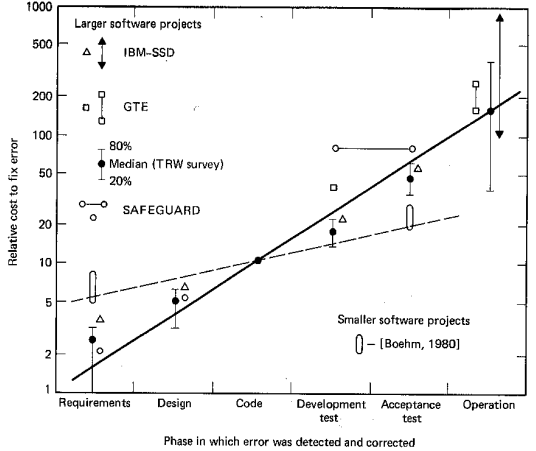
\includegraphics[width=3.3in]{img/boehm_cost-to-fix.png}
 \caption{Historical cost-to-fix curve. From~\cite{Boehm81}.}\label{fig:cost-to-fix}
 \end{figure}
 
In the 40 years since these initial studies, few studies have explored the difficulty to resolve issues
as a function of lifecycle phase. 
Shull et al.~\cite{Shull02} conducted a literature survey and held a series of e-workshops with industry experts on fighting defects. Workshop participants from Toshiba and IBM reported cost-to-fix ratios between early lifecycle and post-delivery defects of 1:137 and 1:117 for large projects respectively~\cite{Shull02} -- but we note here that the raw data points were not provided (which makes confirming those numbers 
a difficult task). 

This was a common theme in the literature reviewed for this paper-- i.e.  that  it was no longer possible to access
the data used to make prior conclusions.
As an example of this, \fig{steck} shows one 2004 survey that reports an exponential delayed issue  effect for 
requirements issues in eight case studies. The right-hand-side of that column shows which of those referenced studies
we can still access-- and a ``?'' denotes a references from a broken url link (note that most
of those links are broken). Note that nearly all of that data is now no longer accessible.


As to the research into agile methods, one goal of that approach
is to reduce the difficulty associated with making changes later in the lifecycle~\cite{beck00}. Relatively little empirical data exists on this point.Elssamadisy and Schalliol~\cite{Elssamadisy02} anecdotally report on the growing, high cost of rework in a 50 person, three-year, 500KLOEC Extreme Programming project as the project grew in size and complexity-- but again we cannot access their 
exact figures.


 
% We note that previous work focuses on cost-to-fix as a function of lifecycle phase irrespective of when the defect was injected, that is, previous work analyzes the cost to fix a defect found in test regardless of whether that defect was a requirements error or a coding mistake. To our knowledge, our research represents the first large-scale study of phase delay.


 \begin{figure}
{\small
\begin{center}
\begin{tabular}{r|rrrr|c}
 case& \multicolumn{4}{c|}{Phase Requirements Issue Found }&  \\
 study               &Requirements & Design & Code&  Test& source\\\hline
1 & 1& 6& 10& 70&~\cite{Boehm81}\\  
2& 1 &3& 5& 37&?\\ 
3&  1 &3& 7& 51& ?\\ 
4& 1& 5 &33 &75& ? \\
5& 1  &    & 10 & 40& ?\\ 
6& 1   &    & 10 &  40& ?\\
7&  1 & 20 & 45 & 250& ?\\  
8&  1  &   5 &      & 50& ? \\\hline
median           & 1 &  5  & 10   & 50.5 
\end{tabular}
\end{center}}
\caption{Sample of the Stecklein et al. literature review~\cite{steck04}:
cost to resolve requirements issues, relative to resolving issues during requirements.
Question marks ``?'' denotes a reference to
a result that is not longer accessible (i.e. a broken URL link).}\label{fig:steck}
\end{figure}


\begin{figure}[!b]
 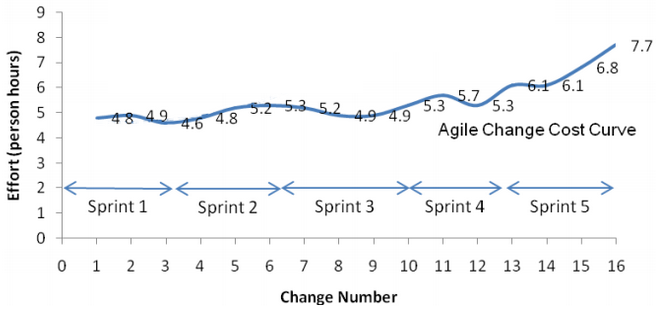
\includegraphics[width=3in]{img/clutterbuck.png} 
 \caption{Cost of change from an agile case study. From~\cite{Clutterbuck09}.}\label{fig:clutterbuck}
 \end{figure}

 
 
 All in all, the empirical results of this section seem insufficient to justify
 the widely-held beliefs documented in the previous section. Adding to our doubts
 was the discovery of at least two studies that report less-than exponential
 increase in the difficulties associated with making the changes associated with delayed
 issues. For example,
Clutterbuck et al.~\cite{Clutterbuck09} studied 5-month effort by a small-to-medium enterprise team developing a 71KLOEC web interface to a database application to implement 18 change requests-- see Figure~\ref{fig:clutterbuck} (note that these were for new and changed user requirements, not defects). Clutterbuck et al. found the cost of change to be relatively flat until the later phases, with much of the effort spent in analysis of the change requests~\cite{Clutterbuck09}. Note that in this study, the effort increased by only 60\% (see the start and end of the curve in Figure~\ref{fig:clutterbuck}).



\begin{figure}
 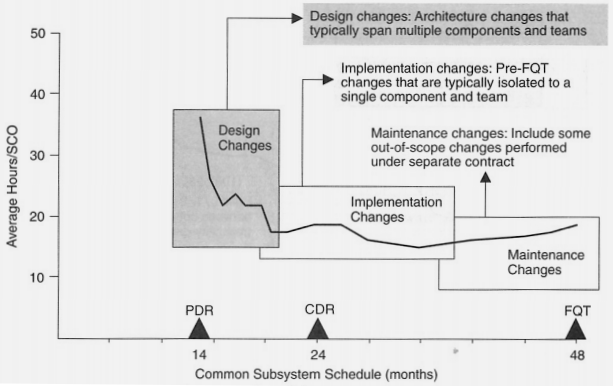
\includegraphics[width=3.3in]{img/Royce98.png}
 \caption{Exception to the rule - CCPDS-R case study cost-to-fix curve. From~\cite{Royce98}.}\label{fig:royce}
 \end{figure}
 
Another example of less-than exponential explosion in the difficulty associated with delayed issues comes from the  CCPDS-R
system described by Royce~\cite{Royce98}. This was a million-line, safety-critical missile defense system show in Figure~\ref{fig:royce}. In this project, design changes (including architecture changes) required approximately twice the effort of implementation and test changes, and the cost-to-fix in implementation and test phases increased slowly. Boehm~\cite{Boehm10} attributes this success to the CCPDS-R development process, which focused on removing architecture risk early in the development lifecycle.
 